\documentclass[14pt]{beamer}
\setbeamertemplate{itemize item}{$\bullet$}
\setbeamertemplate{navigation symbols}{}
\setbeamertemplate{mini frames}{}
\setbeamertemplate{section in toc}[sections numbered]
\setbeamertemplate{itemize items}[square]
\setbeamercolor*{item}{fg=gray}
\usecolortheme{dove}
\hypersetup{pdfpagemode=FullScreen}

\usepackage[T1]{fontenc}
\usepackage[utf8]{inputenc}
\usepackage[yyyymmdd]{datetime}

% Define some accent colours:
\definecolor{DarkFern}{HTML}{407428}
\definecolor{DarkCharcoal}{HTML}{4D4944}
\colorlet{Fern}{DarkFern!85!white}
\colorlet{Charcoal}{DarkCharcoal!85!white} 
\colorlet{LightCharcoal}{Charcoal!50!white}
\colorlet{AlertColor}{orange!80!black}
\colorlet{DarkRed}{red!70!black}
\colorlet{DarkBlue}{blue!70!black}
\colorlet{DarkGreen}{green!70!black}
\definecolor{palecerulean}{rgb}{0.61, 0.77, 0.89}

% Use the colours:
\setbeamercolor{alerted text}{fg=palecerulean}
\setbeamercolor{title}{fg=blact}

% Create horizontal rule, header, and title page
\makeatletter
\def\vhrulefill#1{\leavevmode\leaders\hrule\@height#1\hfill \kern\z@}
\makeatother
\setbeamertemplate{frametitle}{\color{black}\bfseries\insertframetitle\par\vskip-6pt\color{palecerulean}\vhrulefill{1.75pt}}
\defbeamertemplate*{title page}{customized}[1][]
{
	{\begin{centering}
	\usebeamerfont{title}\bfseries\inserttitle\par\bigskip
	\usebeamerfont{subtitle}\insertsubtitle\par\vskip-3pt\color{palecerulean}\vhrulefill{1.75pt}\color{black}\\
	\bigskip
	\bigskip
	\usebeamerfont{author}\insertauthor\par\bigskip
	\usebeamerfont{institute}\insertinstitute\par
	\usebeamerfont{date}\insertdate\par
	\usebeamercolor[fg]{titlegraphic}\inserttitlegraphic
				\insertframetitle\par
	\smallskip\end{centering}}
}


\title{L'écologie au Canada}
\subtitle{Le bien, le mal et le pire}
\author{Anthony Kevins}
\date{\today}


\begin{document}

\begin{frame}
\titlepage
\end{frame}

\begin{frame}
	\frametitle{L'élément déclencheur}
	\begin{figure}
		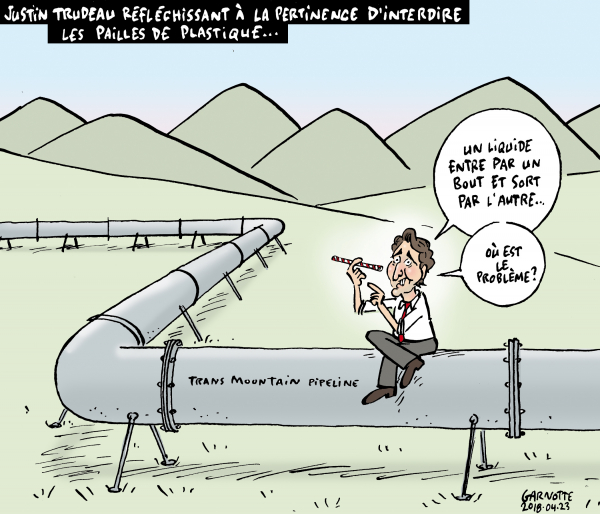
\includegraphics[scale=.575]{trans_mountain}
	\end{figure}
\end{frame}

\begin{frame}
\frametitle{Le bien}
« Le Canada est de retour. Nous sommes là pour vous aider. Pour construire un accord dont nos enfants et nos petits-enfants pourront être fiers. » - Trudeau, 2015 (Paris)

\bigskip

\begin{itemize}
	\pause
	\item L'Accord de Paris % Pousser pour 1.5 degré. Rôle de "leader" 
	\pause
	\item La taxe carbone % À 20, puis ira à 50 en 2022. Ça devrait être à 92 pour être efficace   
	\pause
	\item L'infrastructure % Banque d'infrastructure, avec le privé. Investissements dans le transport en commun 
	\pause
	\item Le plastique % Thème pour son année du G7. Plastique à usage unique serait interdit dès 2021. 
\end{itemize}

\end{frame}

	\begin{frame}
		\frametitle{Le mal} 
	« Aucun pays ne laisserait dans son sol 173 milliards de barils de pétrole sans les exploiter. » - Trudeau, 2017 (Houston)
	
	\bigskip

		\begin{itemize}
			\pause
			\item Les sables bitumineux % un mélange de bitume brut, qui est une forme semi-solide de pétrole brut, de sable, d'argile minérale et d'eau 
			\pause
			\item 3 à 10 fois plus polluant % par baril que le pétrole standard. 
			\pause
			\item Peu rentable % beaucoup moins convoité, de pire qualité
			\pause
			\item Les subventions % 54 milliards en 2018, un léger recul depuis 2015 (58 milliards)
			\pause
			\item Les oléoducs % Gouvernement a acheté le Trans Mountain pour 4,5 milliards. Compte investir 5 milliards de plus puis de le revendre. 
		\end{itemize}
	\end{frame}


	\begin{frame}
		\frametitle{Le pire}
		« On a trouvé le juste équilibre. » François-Philippe Champagne, Ministre fédéral de l’Infrastructure, 2019
		
		\bigskip

		\begin{itemize}
			\pause
			\item Les mêmes cibles qu'avant...
			\begin{itemize}
				\pause
				\item Entre 1990 et 2030 :
				\pause
				\item 40~\% en France, dans l'UE et en Norvège  
				\pause
				\item 15~\% au Canada
			\end{itemize}
			\pause
			\item ... qui sont assez timides... 
			\begin{itemize}
				\pause
				\item 716 millions de tonnes au Canada en 2017, ou 20 par personne
				\pause
				\item 7 par personne en France, 8 dans l'UE, 9 en Norvège
			\end{itemize}
			\pause
			\item et reste hors de portée...  
			\begin{itemize}
				\pause
					\item Augmentation de 116 millions de tonnes par rapport à 1990, 8 l'année passée
			\end{itemize}
		\end{itemize}
	\end{frame}

	\begin{frame}
		\frametitle{Conclusion} 
	« Si le Canada devait consulter un psychologue, ce serait pour schizophrénie aiguë. » - Daniel Green, Chef adjoint du Parti vert, 2019
	
	\bigskip

		\begin{itemize}
			\pause
			\item Redorer notre blason
			\pause
			\item Cadre de réference : les É.-U. et... c'est tout
			\pause
			\item Changements à la marge
			\pause
			\item Le sentiment d'être vertueux 
			\pause
			\item Continuité fondamentale 
		\end{itemize}
	\bigskip
	\pause
	Vers plus d'action, ou moins ?
\end{frame}

\end{document}
